\chapter{Evaluation}
\label{chapter:evaluation}
  In the previous chapter we described how we implemented our solution namely the data model that we used, the description of the signaling protocol, how we performed stream recording, how we overlayed interactive content to video. 

  In this chapter we describe how we deployed our solution, tested our prototype, show and analyze the results in order to validate the contributions of this thesis.

\section{Solution deployment}
	\label{section:deployment}

	In this section we describe the hardware and software we have used to deploy our solution. 

	\subsection{Hardware}

	The hardware was gently provided by INESC-ID\footnote{\url{http://www.inesc-id.pt/} (Accessed March 26, 2016)}, the specifications of the server that we used are specified on table \ref{table:hwspecs}.

	\begin{table}[!htb]
\centering
\caption{Hardware specifications}
\label{table:hwspecs}
\begin{tabular}{|l|l|}
\hline
Server & Supermicro SuperServer 6027R-72RF\footnotemark \\ \hline
CPU & 2 x Intel Xeon E5-2640V2, LGA 2011, 2.0GHz, 8C/16T \\ \hline
RAM & 8 x DDR3 REG16G-1600DDR3, 16GB, DDR3-1600, Registered ECC, memory \\ \hline
Network cards & 2 x Intel Corporation I350 Gigabit Network Connection (rev 01)  \\ \hline
Disks & \begin{tabular}[c]{@{}l@{}}2x SAMSUNG SSD 840 PRO 256GB SATA III (Drive 0 - RAID 1 - 237.486 GB)\\
4x WESTERN DIGITAL 3TB SATA III 64MB RED (Drive 1 - RAID 5 - 8.185TB)\end{tabular} \\ \hline
\end{tabular}
\end{table}

 \footnotetext{\url{http://www.supermicro.com/products/system/2U/6027/SYS-6027R-72RF.cfm} (Acessed March 26, 2016)}

\subsection{Operating System}
	
On table \ref{table:osspecs} we present an overview of the operating system configurations of the machine we used for deployment.

	\begin{table}[!htb]
\centering
\caption{Operating system specifications}
\label{table:osspecs}
\begin{tabular}{|l|l|}
\hline
Operating System & Linux version 3.16.0-4-amd64 \\ \hline
Distribution & Debian GNU/Linux 8 (jessie)\footnotemark \\ \hline
Swap & 16GB (Drive 0)\\ \hline
Root & 40GB (Drive0)\\ \hline
EFI & 200MB (Drive 0)\\ \hline
Bcache & Remaining space (Drive 0 \& Drive 1) \\ \hline
\end{tabular}
\end{table}

\footnotetext{\url{https://www.debian.org/} (Accessed March 26, 2016)}

\subsection{Software}
	\emph{INESC-ID} provided us a restricted \emph{Linux} account without administration permissions, which we prevented us the installation of our solution directly on the machine because we would need administrative privileges to install all the software that our solution depends on. Although that limitation, they provided access to Docker\footnote{\url{https://www.docker.com/} (Accessed March 27, 2016)} which run on host operating system as an isolated process in user space.

	Inside a Docker container we have the administrative privileges to install all the software dependencies.

	We could use one docker image for each component but in order to reduce the network usage we preferred to install all the components within the same image. At the same we provide an all-in-one easy to deploy solution as all the \ac{IP}s are local.

	We present, on table \ref{table:softspecs}, the software we have installed inside our docker container including the versions that are in use.

	\begin{table}[!htb]
\centering
\caption{Installed Software}
\label{table:softspecs}
\begin{tabular}{|l|l|}
\hline
\multicolumn{1}{|c|}{\textbf{Name}} & \multicolumn{1}{c|}{\textbf{Version}}         \\ \hline
Ubuntu Server\footnotemark & 14.04 LTS   \\ \hline
Oracle Java & 1.8.0\_77   \\ \hline
Play Framework & 2.5.0  \\ \hline
MongoDB & 3.0.10   \\ \hline
Kurento Media Server & 6.4.0 \\ \hline
Kurento Repository & 6.3.1 \\ \hline
Python & 2.7.6 \\ \hline
\end{tabular}
\end{table}
 \footnotetext{\url{http://www.ubuntu.com/} (Accessed March 27, 2016)}






\section{Tests Objectives}

  We have tested our solution with real users for a better understanding of their difficulties and what can be done in order to improve our solution's usability.

  We have also tested the performance of our solution by measuring the used resources. Those performance tests are crucial to ensure that our solution is in fact stable and users can use it endlessly without decreasing the quality of their experience. 


  \section {Performance Tests}

     In this section we describe performance tests that we have applied and their respective results.


    \subsection{Tests Scenarios}


      In order to benchmark our system, we have implemented a small \emph{Python} script using \emph{psutil}\footnote{\url{https://github.com/giampaolo/psutil} (Accessed March 27, 2016)} that collects with a periodicity of one second: CPU, physical memory information relative to each running process and network usage relative to each interface. 

      We would like to collect network information relative to each process, which \emph{nethogs}\footnote{\url{https://raboof.github.io/nethogs/} (Accessed March 27, 2016)} provide but it could not capture the network usage of some processes. Although this would be useful for a deep analysis, we know which network interfaces are used to establish connections between processes as we show on Table \ref{table:interfacemap}.

  \begin{table}
\centering
\caption{Mapping of connections by network interface}
\label{table:interfacemap}
\begin{tabular}{|l|l|}
\hline
\multicolumn{1}{|c|}{\textbf{Interface}} & \multicolumn{1}{c|}{\textbf{Connection}}         \\ \hline
Loopback & Web Server $\leftrightarrow$ MongoDB  \\ \hline
Loopback & Web Server $\leftrightarrow$ Kurento Media Server  \\ \hline
Loopback & Kurento Media Server $\leftrightarrow$ Kurento Repository $\leftrightarrow$ MongoDB  \\ \hline
Ethernet & Web Server $\leftrightarrow$ Client\\ \hline
Ethernet & Kurento Media Server $\leftrightarrow$ Client\\ \hline
\end{tabular}
\end{table}


      The performance test scenario that we have defined consists on two phases, the first phase consists only on having users, with similar computer and network specifications, entering sequentially on the conference room. The second phase consists on the users leaving the conference room. Each event, joining and leaving, occurs with intervals of one minute in total of thirteen minutes (780 seconds).

  


\subsection{Test Results}
  
      In this section we discuss the results of our performance tests performed after implementing our solution.
\subsubsection{Network usage}

      Every time a user shares its camera or its screen in the context of a conference room, its offered video is sent to the server and, independently from watching an individual stream or the mixed version, the server just sends a unique stream back to the user.

      From the media server perspective if there are $n$ clients connected, each of them sending and receiving one stream, it is expected that server sends and receives also $n$ streams. As such, we expect that the amount of network traffic increases linearly as users join a conference room. Figure \ref{fig:test_full_features_net} confirms our expectations. Each vertical yellow line represents one event: the first seven events are users entering the conference room, the next ones represent users leaving the conversation. 
      

\begin{figure}
  \centering
  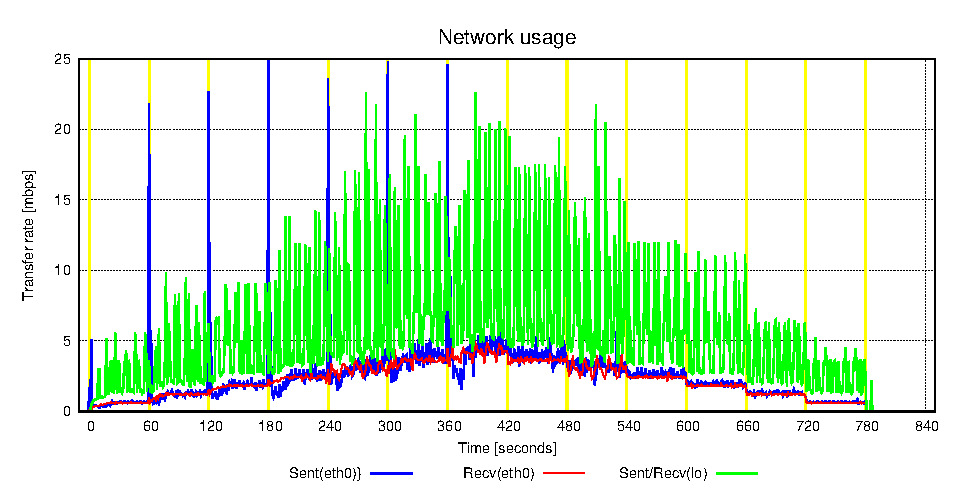
\includegraphics[width=\textwidth]{stats/test_full_features_net.eps}
  \caption{Network usage after implementing all features}
  \label{fig:test_full_features_net}
\end{figure}


      The blue peaks are caused by the signaling phase and web page downloads, including resources such as images, stylesheets and javascript files. 
      The green peaks are caused by video and audio being transfered between \ac{KMS} and \emph{MongoDB} through \emph{Kurento Repository}. Each peak occurs every time a block of video is recorded, which in this case is every ten seconds. 
      The recordings are synchronized so all user and mixed blocks start and end at the same time. That is why the amount of work done every ten seconds accumulates, and because this is performed locally, the maximum transfer rate is limited by the performance of the memory as buffers are written to buffers then to disks. 
      Sent data transfer rate has no significant peaks as \ac{HTTP} requests and signaling information contains little information.

      Figure \ref{fig:summary_full_net} shows the average transmission rate per interval of consecutive events. 


\begin{figure}
  \centering
  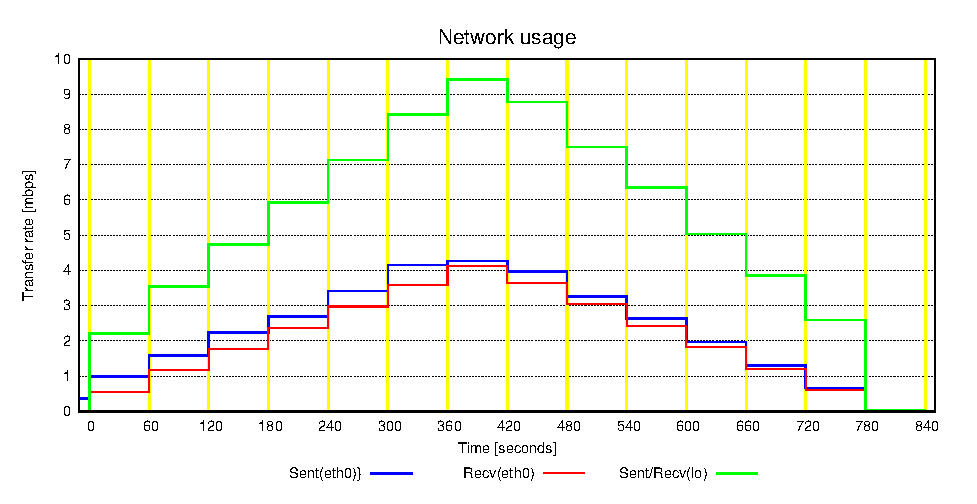
\includegraphics[width=\textwidth]{stats/summary_full_net.eps}
  \caption{Average network usage per interval of events after implementing all features}
  \label{fig:summary_full_net}
\end{figure}



If we consider all streams equal and an incoming stream uses $x$kbps, with $n$ incoming streams the rate of data received at \ac{KMS} is $nx$ and the expected rate of data transfered to \emph{Kurento Repo} using localhost is $(n+1)x$. Due to the data being transfered also from \emph{Kurento Repo} to \emph{MongoDB} via localhost, the expected total rate of data transfered through localhost is $2((n+1)x) = (2n+2)x$, which explains the reason for the average amount of data transfered through localhost being more than twice the average amount of data received from users.

With this results we conclude that if we want to scale our storage solution using the \emph{MongoDB}'s cluster configuration, both \emph{Kurento Repository} and \ac{KMS} should be installed on the same machine, as depicted on figure \ref{fig:scale2}, because the loopback interface can handle bigger transfer rates than the remaining network interfaces. Installing the repository on the same machine as a database node does not ensure that recorded videos are stored in the same machine, for this reason we would prefer installing \ac{KMS} and \emph{Kurento Repository} on the same machine.

\begin{figure}
  \centering
  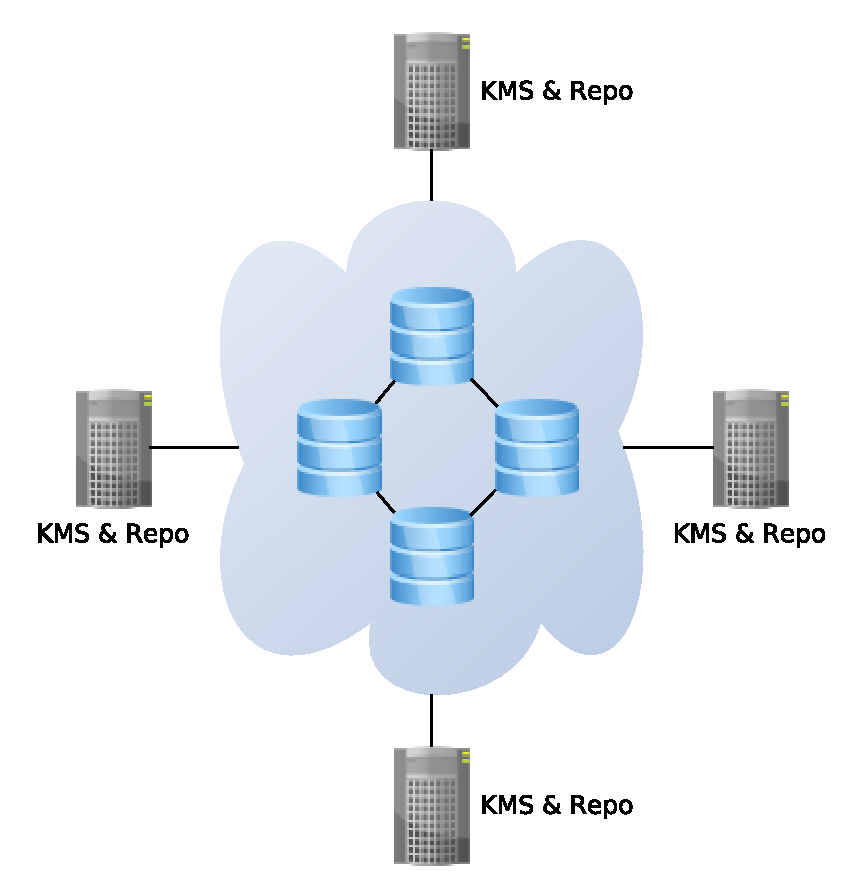
\includegraphics[width=0.5\textwidth]{figures/scale2.pdf}
  \caption{Repository and KMS in the same machine}
  \label{fig:scale2}
\end{figure}



On the other hand, Figure \ref{fig:test_client_net} shows the respective network usage on the client side during our test case. We observe that in the first seconds the client adjusts the video quality it sends to \ac{KMS}. Whenever a new client enters the conference, we observe that \ac{KMS} decreases the video quality in order to instantaneously integrate a new user into the conference room. After a while, \ac{KMS} realizes that the network can handle the increase of clients and sends the video with a better quality to every participant. When a user leaves the conference room \ac{KMS} has no need to decrease the participant's video quality as less network bandwidth will be used.

\begin{figure}
  \centering
  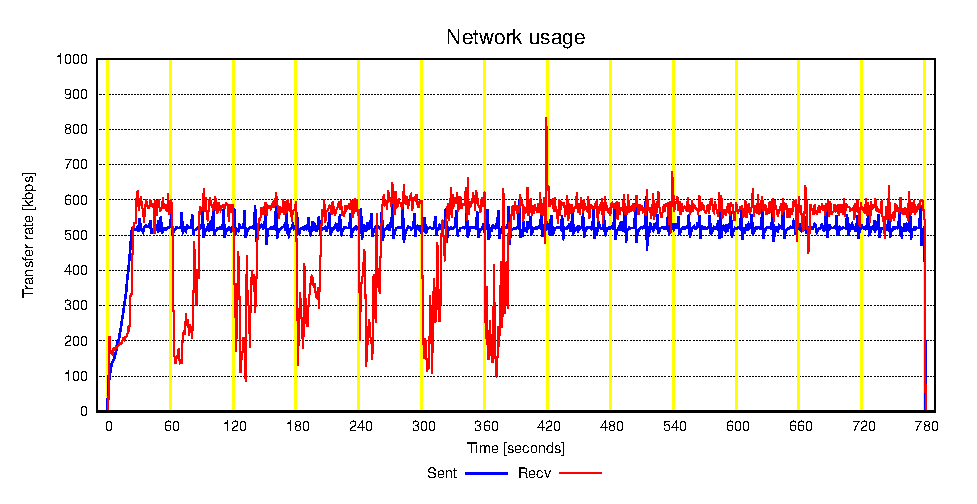
\includegraphics[width=\textwidth]{stats/test_client_net.eps}
  \caption{Client Network usage during our test case}
  \label{fig:test_client_net}
\end{figure}



\subsubsection{Memory usage}


Figure \ref{fig:test_full_features_mem} shows the memory usage during our performance test. Both \ac{JVM}, \emph{MongoDB} and \ac{KMS} performs their own memory management by holding and recycling objects when needed. The expected and observed behavior of the memory usage is growth of memory usage while the users are entering the conference room and a memory usage stabilization afterwards.



\begin{figure}
  \centering
  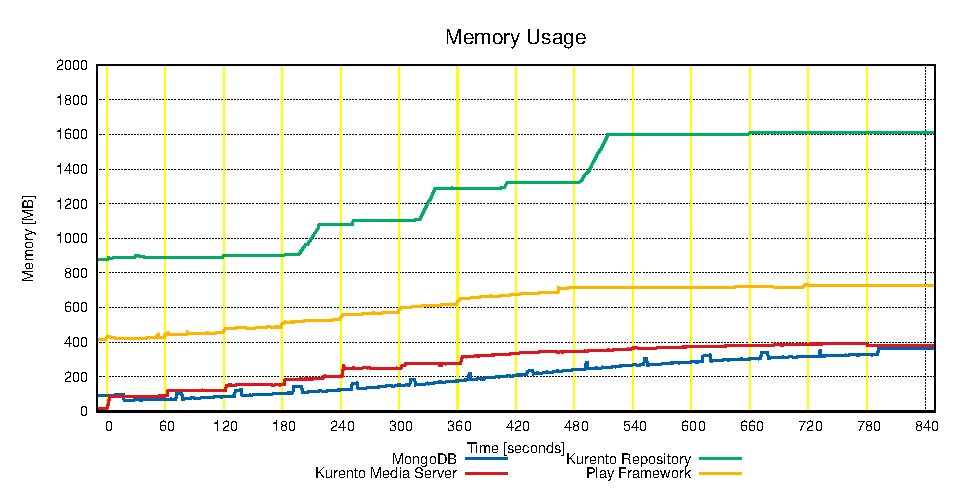
\includegraphics[width=\textwidth]{stats/test_full_features_mem.eps}
  \caption{Memory usage after implementing all features}
  \label{fig:test_full_features_mem}
\end{figure}


\emph{MongoDB} memory usage keeps increasing because it tries to fit part of the database on \ac{RAM} for fast read access. \emph{MongoDB} checkpoints data to disk every 60 seconds or when journal data exceeds 2GB\footnote{\url{https://docs.mongodb.org/manual/faq/storage/}(Accessed March 28, 2016)}, that explains the small memory usage peaks during our test case. When the conference room is empty there are no video recordings, which explains the memory stabilization at the end.

\emph{KMS} memory usage was increasing and in fact we did not expected that. We have done more tests and we have observed that by disabling the recorder feature, memory usage kept linearly related to the amount of clients present on the room. Therefore, we have verified our implementation and we have concluded that nothing was wrong with our code: we have confirmed that every allocated resource was indeed released after the end of recording. As a result of our intensive tests and consecutive failures we suspected that the problem was not ours.

Hence, in order to confirm our suspicions, we have decided to read the implementation of \ac{KMS} and we have found that \ac{KMS} was not releasing the memory if the recorder was stopped by us. Subsequently, we have changed the source code and submitted to \emph{Kurento} team through a \emph{GitHub}'s \emph{"pull request"}, which was accepted.


Figure \ref{fig:test_ram_fixed_mem} shows the memory usage during our performance test case using the patch that we applied to \ac{KMS}. As we can observe, there were \ac{KMS} and also \emph{Kurento Repository} memory usage improvements. 



\begin{figure}
  \centering
  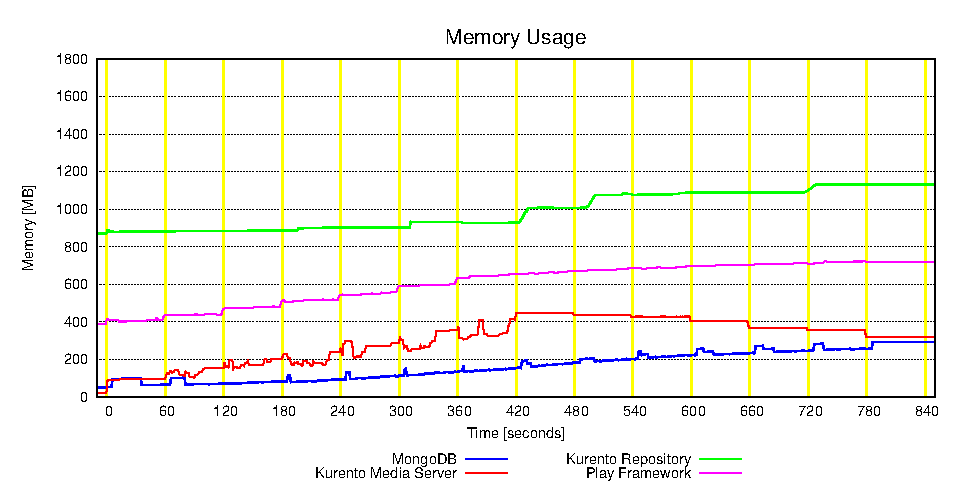
\includegraphics[width=\textwidth]{stats/test_ram_fixed_mem.eps}
  \caption{Memory usage after fixing recorder memory leak}
  \label{fig:test_ram_fixed_mem}
\end{figure}


\subsubsection{CPU usage}


Figure \ref{fig:test_full_features_cpu} shows the percentage of \ac{CPU} usage during our performance test case. Each 100\% represents one \ac{CPU} core, although that does not mean one \ac{CPU} is fully used, for example two cores at 60\% represent 120\% \ac{CPU} usage. As we can see, the percentage of \ac{CPU} used increases and decreases linearly in function of the amount of conference participants. 

\begin{figure}
  \centering
  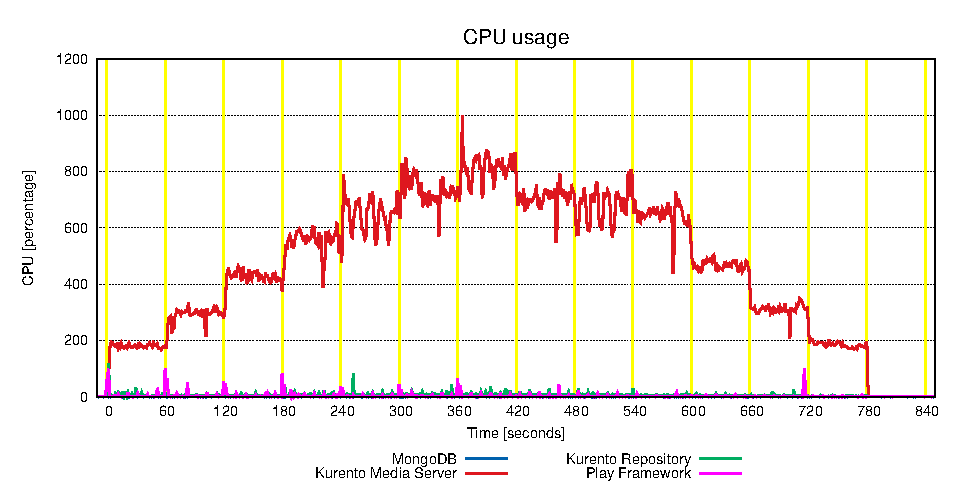
\includegraphics[width=\textwidth]{stats/test_full_features_cpu.eps}
  \caption{Percentage of CPU used during the performance tests}
  \label{fig:test_full_features_cpu}
\end{figure}

Figure \ref{fig:test_full_features_cpu_zoom} is the same as figure \ref{fig:test_full_features_cpu} but zoomed over \emph{MongoDB}, \emph{Java} and \emph{Kurento Repository}. As we can see there are periodic processing peaks every ten seconds that are due to block recording. \ac{KMS} is responsible for most \ac{CPU} usage.

\begin{figure}
  \centering
  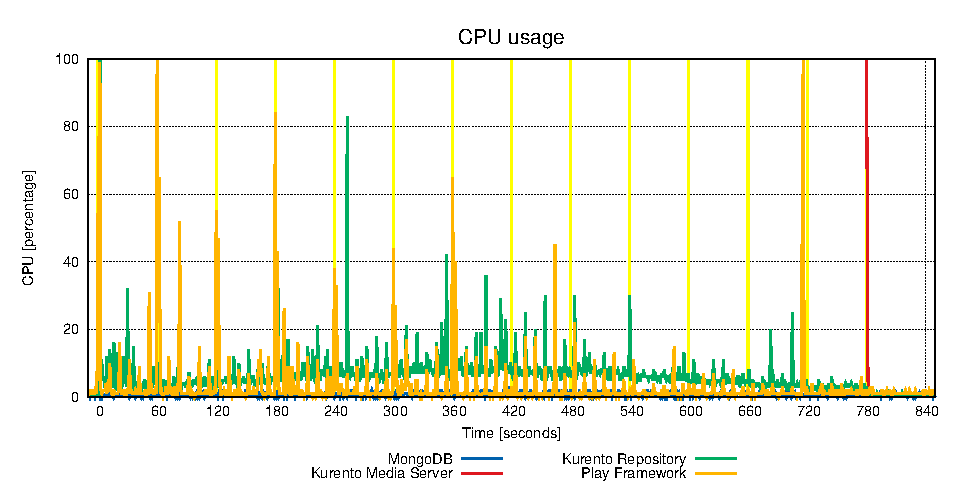
\includegraphics[width=\textwidth]{stats/test_full_features_cpu_zoom.eps}
  \caption{Percentage of CPU used during the performance tests (zoomed)}
  \label{fig:test_full_features_cpu_zoom}
\end{figure}


   Figure \ref{fig:summary_full_cpu} shows the average used \ac{CPU} per interval of consecutive events. 

\begin{figure}
  \centering
  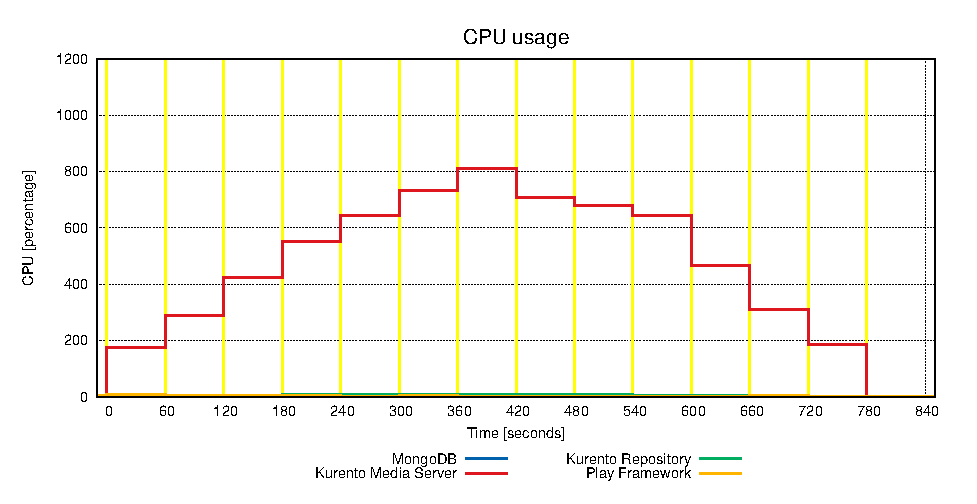
\includegraphics[width=\textwidth]{stats/summary_full_cpu.eps}
  \caption{Average percentage of CPU used per interval of events after implementing all features}
  \label{fig:summary_full_cpu}
\end{figure}



  Just for testing purposes, we performed the same performance tests disabling \ac{QR} codes detection in order to understand how \ac{CPU} intensive this task is. Figure \ref{fig:test_without_qrcode_cpu} shows the results for the same experience but with \ac{QR} code detection disabled.

\begin{figure}
  \centering
  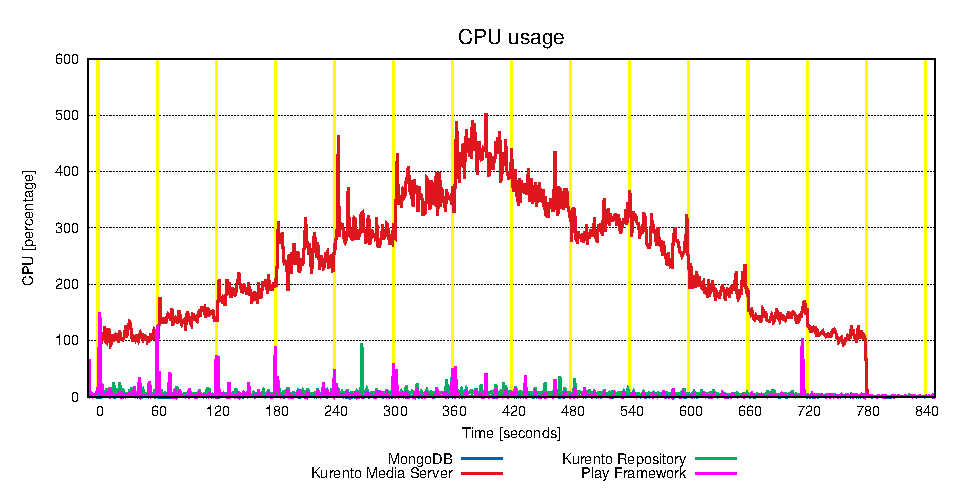
\includegraphics[width=\textwidth]{stats/test_without_qrcode_cpu.eps}
  \caption{Percentage of CPU used during the performance tests without QR code detection}
  \label{fig:test_without_qrcode_cpu}
\end{figure}

We conclude that \ac{QR} code detection is a very intensive task, approximately doubling the amount of work performed by the \ac{CPU}s. Without this feature, the network and memory usage had insignificant changes compared to \ac{CPU} usage.

Even though, with this test results, we conclude that our solution's bottleneck is the \ac{CPU} usage at \ac{KMS}.

\subsubsection{Two consecutive test cases}


We have also performed two consecutive test cases in order to understand if we the influence of the first test case over the second, as observed in figure \ref{fig:test_two_times_cpu}, there is no \ac{CPU} influence between two test cases.


\begin{figure}
  \centering
  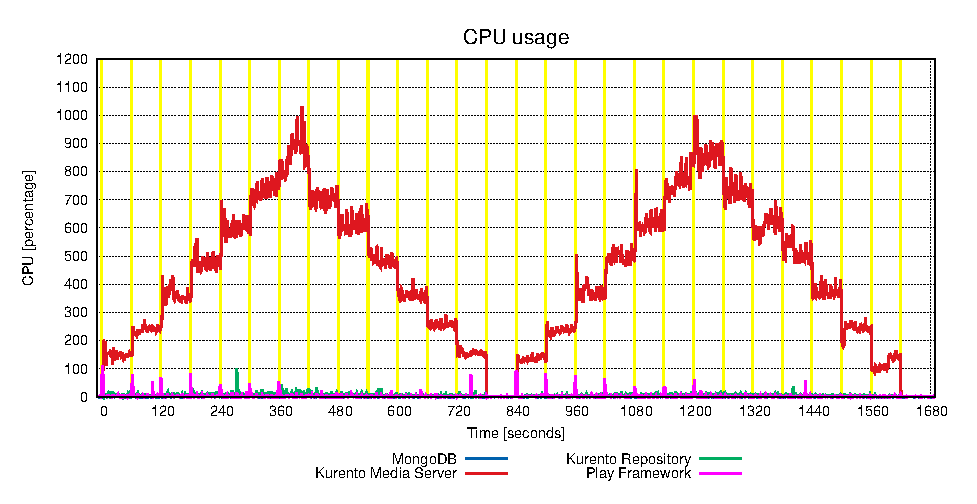
\includegraphics[width=\textwidth]{stats/test_two_times_cpu.eps}
  \caption{Percentage of CPU used during two consecutive test cases}
  \label{fig:test_two_times_cpu}
\end{figure}

On the other hand due to memory recycling techniques we can observe in figure \ref{fig:test_two_times_mem} that some of the memory that was allocated in the first test was reused in the second case.


\begin{figure}
  \centering
  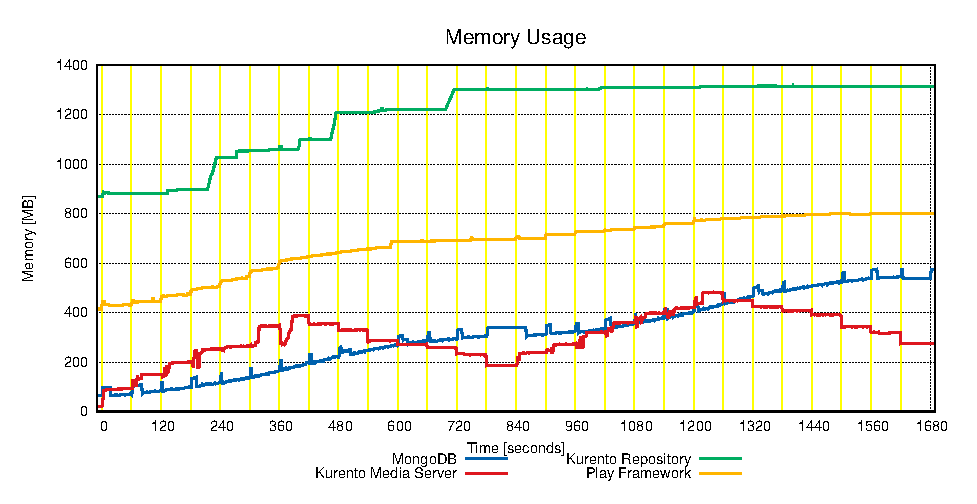
\includegraphics[width=\textwidth]{stats/test_two_times_mem.eps}
  \caption{Memory usage during two consecutive test cases}
  \label{fig:test_two_times_mem}
\end{figure}


\subsubsection{One hour test case}


   Figure \ref{fig:test_hour_mem} shows the memory used by our solution with seven clients simultaneously on the same conference room during one hour. As we can observe, \ac{KMS} memory usage stabilizes.


\begin{figure}
  \centering
  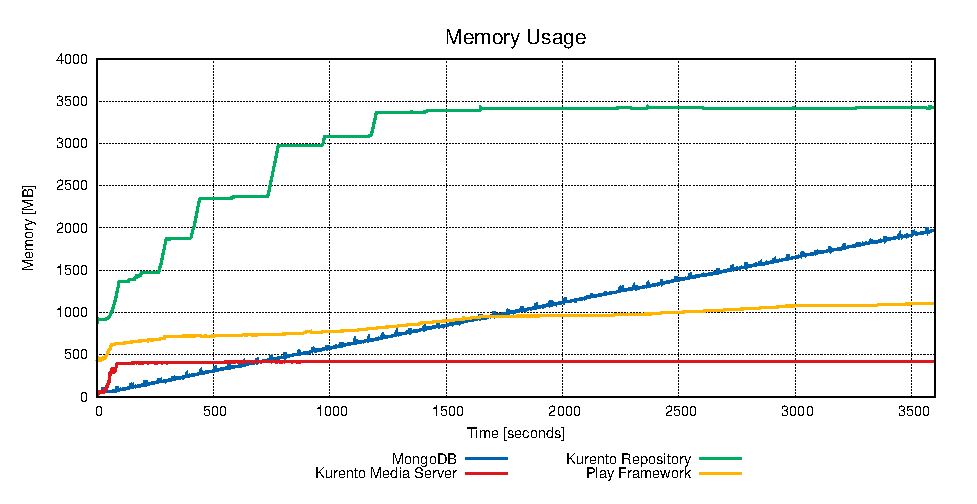
\includegraphics[width=\textwidth]{stats/test_hour_mem.eps}
  \caption{Memory usage during one hour with seven clients}
  \label{fig:test_hour_mem}
\end{figure}





\section {Usability Tests}
     In this section we describe usability test scenarios that we have applied and their respective results.


    \subsection{Tests Scenarios}

      In order to evaluate the usability of our solution, we have performed usability tests with the help of real users with different backgrounds and ages.

      We handed a guide to the users with five tasks to perform. The metrics we used for each task were: number of clicks, number of errors (including a description) and time spent. 

      The tasks we asked the user to perform were:

      \begin{enumerate}
      \item Login into the system with the provided credentials and accept the received friendship request. Find a given user by its name and add him as a friend.

      \item Create a private conference room, enter and share your screen, add the coordinator to the conference room and chat with him. After that use the collaborative editor in order to write at the same time as the coordinator. Lastly save the editor and leave the conference room.

      \item Enter a conference room correspondent as an observer and navigate to the specified annotation. Watch the video until a list of topics is overlayed in the video and choose one of them and leave the conference room.

      \item Enter a conference room by sharing their camera and create a time annotation in the instant of time when they entered, navigate to the current time, search for the annotation and leave the conference room.

      \item Enter a conference room by sharing their camera and add a subtitle in the video, preview it, specify an interval of time and save it. Then show the provided \ac{QR} code to the camera and leave the leave the conference room.
      \end{enumerate}

      The goal of the first task is to evaluating the interface for authentication and friendship management.

      The second task is used to evaluate our tools for collaborative content edition.

      The goal of the third task is to demonstrate the navigation functionalities and synchronized interactive content superposition.

      The fourth task is used to analyse the behavior and difficulties of the user when creating a time annotation.

      The goal of the fifth task is to create synchronized overlayed content and present an easier way to synchronize content.

  \subsection{Test Results}

In this section we present the results of our usability tests. The first time we tested our solution by providing tasks to users, we have observed that our solution was not perfect. Having faced usability problems during our tests, he had to improve our solution's usability and start the tests again.

  \subsubsection {First phase}

In the first testing phase we have performed tests with just three users and ceased for improvements. 

The initial users that tested our solution had difficulties in the first task when finding new friendship requests and adding new friends, as friendship request were only possible to access from the top bar and new user profiles were only accessible through the search bar. In order to solve this problem we have added a menu for adding new users in the friends list and another near the friends list as it can be seen on figure \ref{fig:test_ui_01_02_03}.

\begin{figure}
\centering
\begin{minipage}[b]{0.2\linewidth}
\centering

    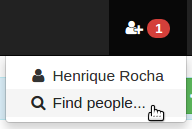
\includegraphics[width=\textwidth]{figures/test_ui_01.png}
        a) Friend list path
\end{minipage}
\begin{minipage}[b]{0.35\linewidth}
    \centering

    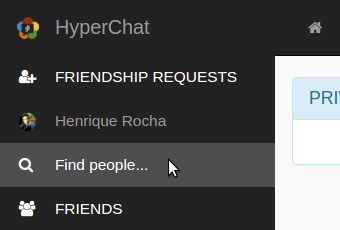
\includegraphics[width=\textwidth]{figures/test_ui_02.png}
         b) Friend requests path
\end{minipage}
\begin{minipage}[b]{0.2\linewidth}
    \centering

    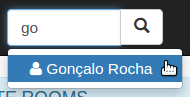
\includegraphics[width=\textwidth]{figures/test_ui_03.png}
         c) Search bar path
\end{minipage}

    \caption{Multiple paths for finding people}
    \label{fig:test_ui_01_02_03}
\end{figure}

On the second task one user clicked on the friends list for adding a friend to a room and, as a consequence, left the conference room to the user profile. We solved this problem by showing a pop-up with the user profile and an additional button to add the user to the conference room as it can be seen on figure \ref{fig:test_ui_04}.

\begin{figure}
\centering
\begin{minipage}[b]{0.7\linewidth}
\centering

    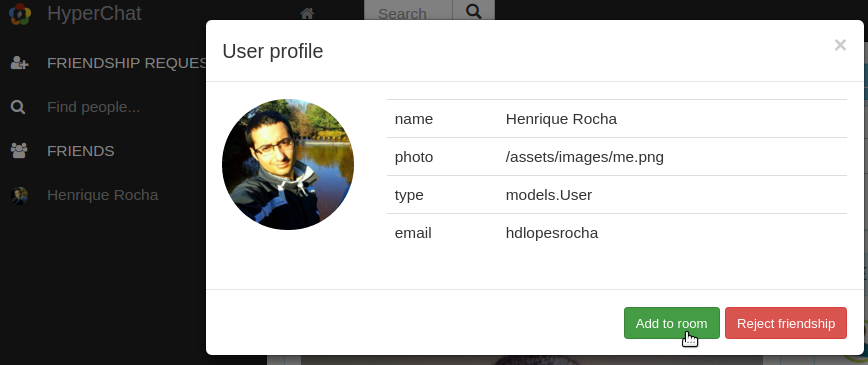
\includegraphics[width=\textwidth]{figures/test_ui_04.png}
\end{minipage}


    \caption{Adding user to conference room from user profile}
    \label{fig:test_ui_04}
\end{figure}

On the third task we noticed that users were not expecting to search the content directly from the search bar, instead they used the time-line.

On the fourth task the users did not placed their annotations on right place. We only provide one way to place annotations, which is by dragging them on the time-line. 
After creating an annotation, users also did not understand that they had to save their changes on the time-line. We solved this problem by saving automatically each time the user changed any annotation. The old user interface can be seen on figure \ref{fig:test_ui_05}.

\begin{figure}
\centering
\begin{minipage}[b]{0.3\linewidth}
\centering

    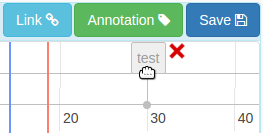
\includegraphics[width=\textwidth]{figures/test_ui_05.png}
\end{minipage}


    \caption{Save button that was removed}
    \label{fig:test_ui_05}
\end{figure}

The three users had success with the fifth task, but they revealed difficulties choosing the time interval for the hyper content. We are aware that this is a difficult task and that's why we have introduced the \ac{QR} code content creation mechanism which was very easy to learn (with a \ac{QR} code already printed into paper).

Although content creation through \ac{QR} codes revealed much easier to perform, this approach implies showing and, as a consequence, recording video with the \ac{QR} codes, making them visible to other users. In order to solve this problem, we could add a new video sharing mode that allow users to send video to \ac{KMS} without composing, recording and showing to other users.

We have also gathered comments and suggestions after letting the users explore our system, extra improvements were made such as:

\begin{itemize}
\item Giving feedback to user when performing operations such as create superimposed content and save the collaborative editor content.
\item Starting with our time-line more zoomed in order to give more sensation of time passing.
\item Create content with starting time and duration, instead of ending time.
\end{itemize}

  \subsubsection {Second phase}

On the second phase of our user interface tests, in a general way, we have noticed great improvements on the learning time.

In order to measure the users learning speed, we have performed tests with experienced users in order to retrieve the optimal task duration and minimal task clicks.

To this end, with regard to optimal task duration and minimal clicks, we obtained the values shown in table \ref{table:optimal}.


\begin{table}[H]
\centering
\caption{Metrics for an experienced user}
\label{table:optimal}
\begin{tabular}{|c|c|c|c|c|c|}
\hline
\textbf{Task} & 1 & 2 & 3 & 4 & 5 \\ \hline
\textbf{Duration (seconds)} & 20 & 35 & 30 & 25 & 35 \\ \hline
\textbf{Number of clicks} & 7 & 10 & 5 & 9 & 7 \\ \hline
\end{tabular}
\end{table}


From the data collected with twenty tests with users, namely the task duration (Figure \ref{fig:user_times}), number of clicks (Figure \ref{fig:user_clicks}), number of errors (Figure \ref{fig:user_errors}), task difficulty (Figure \ref{fig:user_diffs}) and qualitative evaluation (Figure \ref{fig:user_evals}), we have calculated the confidence intervals in order to understand the most plausible values for each metric.

As a result of both true average and variance being unknown and the usage of a relatively small amount of samples, we had to use \emph{t-distribution} to estimate our metrics confidence intervals. 

Accordingly, we have used the following formula to calculate the intervals for the expected value of the true average with 95\% confidence:
\begin{equation}
[\bar{x}-F^{-1}_{t_{(n-1)}}(1-\alpha/2)\times \frac{s}{\sqrt{n}}, \bar{x}+F^{-1}_{t_{(n-1)}}(1-\alpha/2)\times \frac{s}{\sqrt{n}}]
\end{equation}

The youngest and oldest testers were, receptively, twenty two and thirty eight years old. Figure \ref{fig:user_ages} the ages of the users that tested our system.

\begin{figure}
  \centering
  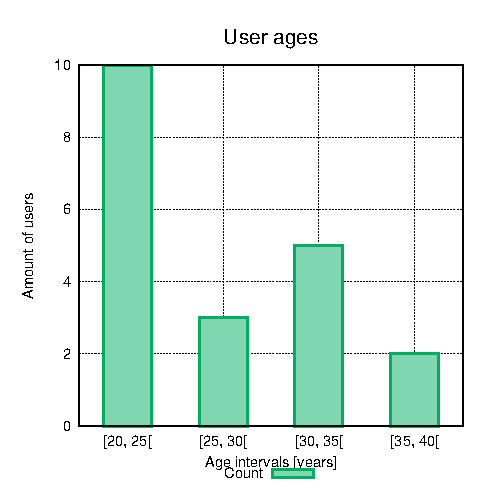
\includegraphics[width=0.5\textwidth]{stats/user_ages.eps}
  \caption{Ages of the users that tested our system}
  \label{fig:user_ages}
\end{figure}


Where $\alpha=0.05$ \footnote{95\% ($\alpha=0.05=1-0.95$) is a common confidence level value used, by researchers, to calculate confidence intervals}, $n$ is the number of samples (which may not coincide with the number of tests due to failed tasks), $\bar{x}$ is the sample mean, $x_i$ is the sample value and $s$ is the sample standard deviation that is given by:
\begin{equation}
s=\sqrt{\frac{1}{n-1}\Sigma^{n}_{i=1}(x_i-\bar{x})^2}
\end{equation}





\begin{figure}
\centering
\begin{minipage}{.5\textwidth}
  \centering
    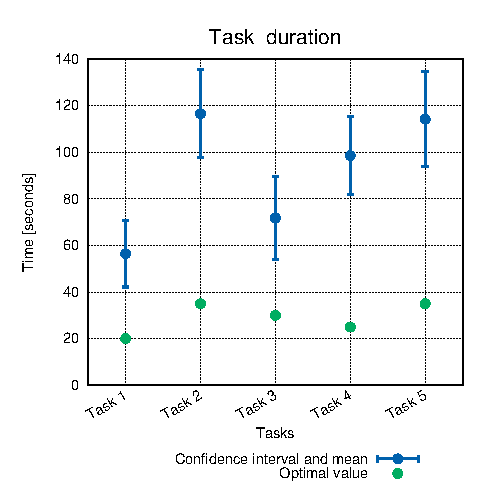
\includegraphics[width=\textwidth]{stats/user_times.eps}
    \caption{Time spent per task}
    \label{fig:user_times}
\end{minipage}%
\begin{minipage}{.5\textwidth}
  \centering
    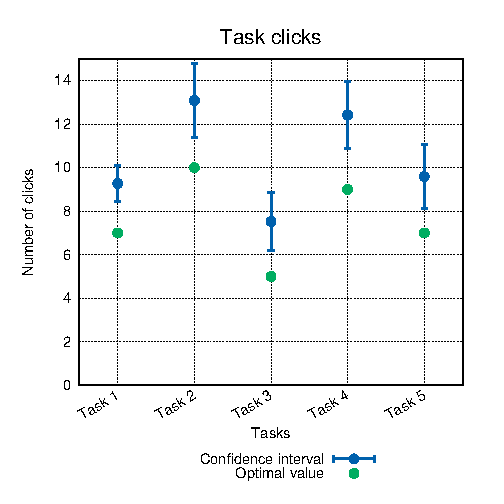
\includegraphics[width=\textwidth]{stats/user_clicks.eps}
    \caption{Mouse clicks per task}
    \label{fig:user_clicks}
\end{minipage}
\end{figure}



According to Figure \ref{fig:user_diffs}, we can observe that most users had less difficulties with the first two tasks, which represents types of tasks that most users are familiar with. As soon as users had to navigate in time, manipulate annotations and create content (respectively \emph{task3}, \emph{task4} and \emph{task5}) we observed that they revealed more difficulties. Most of those difficulties, based on the users feedback, were mainly due to those concepts not being familiar to them.

\begin{figure}
\centering
\begin{minipage}{.5\textwidth}
  \centering
    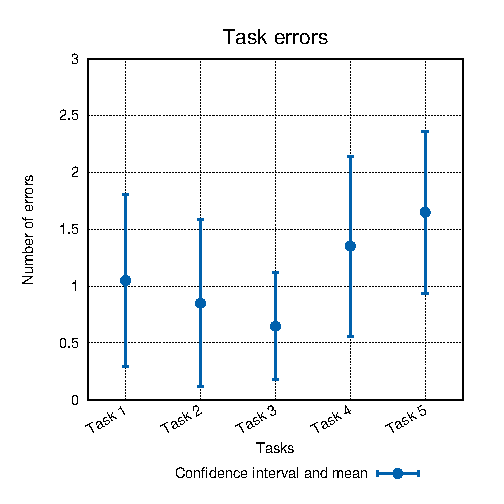
\includegraphics[width=\textwidth]{stats/user_errors.eps}
  \caption{Errors per task}
  \label{fig:user_errors}
\end{minipage}%
\begin{minipage}{.5\textwidth}
  \centering
    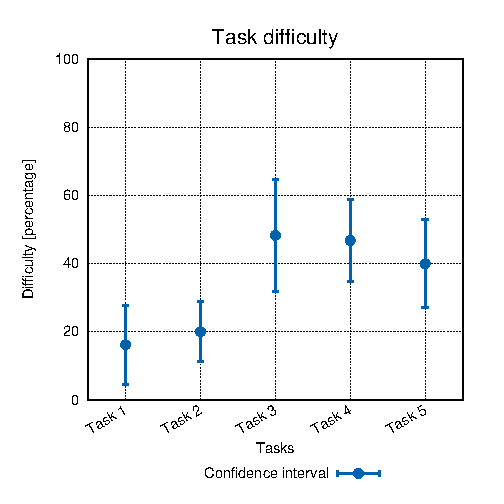
\includegraphics[width=\textwidth]{stats/user_diffs.eps}
  \caption{Difficulty per task}
  \label{fig:user_diffs}
\end{minipage}
\end{figure}


As we had relatively bad results with some users, we explained to those users that could not conclude the tasks or performed them incorrectly, the most efficient way to perform the requested tasks. Some users suggested to display more hints in order to achieve a faster learning, but afterwards all were impressed and gave us a better evaluation (as seen on Figure \ref{fig:user_evals}).

\begin{figure}
  \centering
  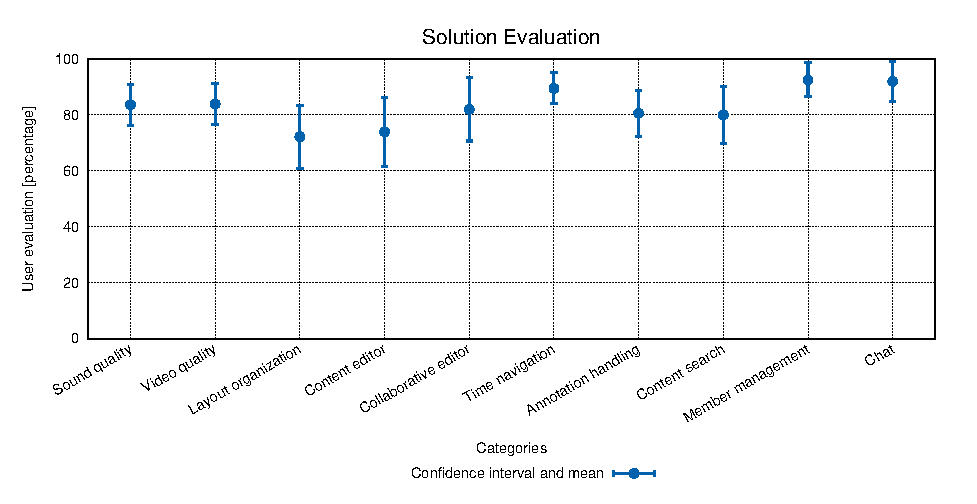
\includegraphics[width=\textwidth]{stats/user_evals.eps}
  \caption{Solution evaluation}
  \label{fig:user_evals}
\end{figure}



Most users gave us worse evaluations on our user interface layout and content editor, which was due to having a lot of tools present in the same web page and some of them being hidden due the screen size. In some cases users had to scroll down in order to find the tools they were looking for. 

Another weak aspect was our content editor, which, in fact, we recognize is difficult to work with, mostly due to the amount of information that is necessary to create a synchronized content (starting time, duration and content itself). Some users have suggested that the content should also be present on the time-line so they could be easily dragged and resized (on time).

We are aware that placing content on the time-line will reduce our solutions performance, especially when there is a relatively large amount of content, due to the content that is present on the time-line being loaded all at once. Although, we recognize that for some cases (relatively low amount of content), displaying the content on the time-line could not have a great impact on our solutions performance, we choose not to implement this.

In conclusion, 100\% of our testers though that our solution was an innovation and 95\% recommended using our solution.


\section{Chapter Summary}
\label{evaluation:summary}

In this chapter we have described how we have deployed our system for allowing a public access and perform tests in a real case environment.
 
Then, we described the test scenarios that we have created in order to evaluate our system. 

The performance tests revealed unexpected results which were crucial to find and solve performance issues. Another important aspect of our performance test results was the understanding of how data flows between our system modules.

In respect to user interface tests, we have obtained valuable feedback that we used to improve our prototype's usability. 

In order to understand how good the results were for each performed task, we have defined optimal values for the different metrics. In general the results reveal a significant difference between observed values and optimal values, which can be explained by the user's lack of experience with systems such as the one we have created.